\begin{frame}{Stan kubitu}

Stan kubitu opisujemy jako wektor w $\mathbb{C}^2$

\[
\ket{\psi}=
\begin{pmatrix}
\psi_1\\
\psi_2
\end{pmatrix}
\]

Warunek normalizacji:

\[
\braket{\psi|\psi}=|\psi_1|^2+|\psi_2|^2=1
\]


Możemy wybrać bazę przestrzeni $\mathbb{C}^2$

\[
\ket{0}=
\begin{pmatrix}
1\\0
\end{pmatrix},
\qquad
\ket{1}=
\begin{pmatrix}
0\\1
\end{pmatrix}
\]
\[\ket{\psi}=a \ket{0} + b \ket{1}\] 
\end{frame}

%================================================


\begin{frame}{Pomiar}
    Mierząc stan \(\ket{\psi}=a \ket{0} + b \ket{1}\) w bazie \(\ket{0}\), \(\ket{1}\)):\\
    \[P(\ket{0})=\braket{0 | \Psi}^2=\left[\begin{pmatrix}
        1 & 0
    \end{pmatrix} \begin{pmatrix}
        a \\ b 
    \end{pmatrix}\right]^2=|a|^2\]

        \[P(\ket{1})=\braket{1 | \Psi}^2=\left[\begin{pmatrix}
        0 & 1
    \end{pmatrix} \begin{pmatrix}
        a \\ b 
    \end{pmatrix}\right]^2=|b|^2\]
    \begin{tikzpicture}[remember picture,overlay]
        \node[anchor=south east, xshift=-0.2cm, yshift=0.2cm] at (current page.south east)
        {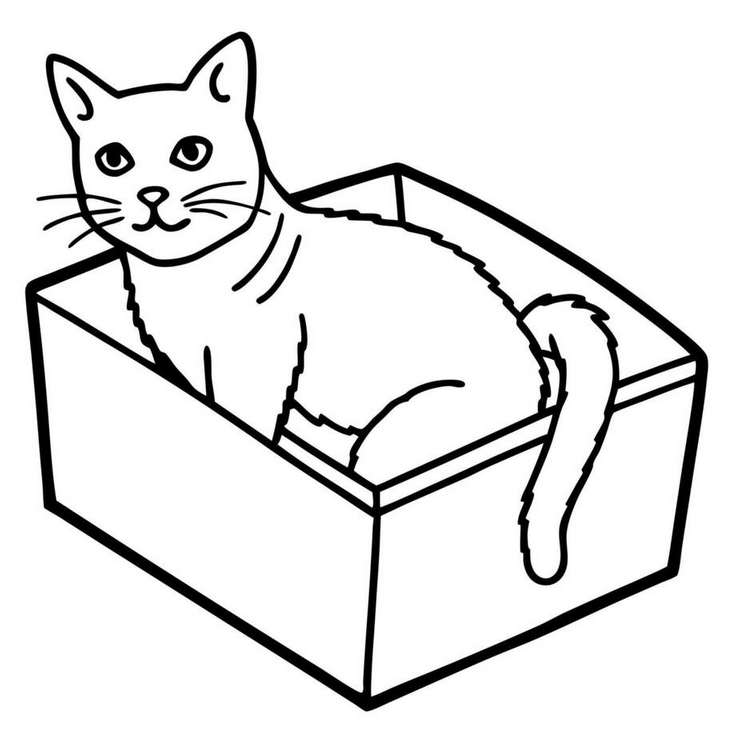
\includegraphics[width=2cm]{images/kotek.png}};
    \end{tikzpicture}
\end{frame}


\begin{frame}{Dowolna baza}
        Dowolną bazę możemy zapisać przy pomocy bazy \(\ket{0}\) \({\ket{1}}\) jako
    \[\ket{\alpha}=\cos \theta \ket{0} + \sin \theta \ket{1}  \qquad \ket{\alpha^\perp}=-\sin \theta\ket{0} + \cos \theta\ket{1} \]
    Wtedy
    \pause
        \[P(\ket{\alpha})=\braket{\alpha | \Psi}^2=\left[\begin{pmatrix}
        \cos \theta & \sin \theta
    \end{pmatrix} \begin{pmatrix}
        a \\ b 
    \end{pmatrix}\right]^2=(a\cos \theta + b\sin \theta)^2\]
\end{frame}

%================================================


\begin{frame}{Iloczyn tensorowy}
Iloczyn tensorowy definiuje wspólny stan dwóch kubitów
\[
\ket{\psi_1} = \begin{pmatrix} a \\ b \end{pmatrix} = a\ket{0} + b\ket{1}, \quad
\ket{\psi_2} = \begin{pmatrix} c \\ d \end{pmatrix} = c\ket{0} + d\ket{1}
\]
\[
\ket{\psi_1 \psi_2}=\ket{\psi_1} \otimes \ket{\psi_2} =
\begin{pmatrix} a \\ b \end{pmatrix} \otimes 
\begin{pmatrix} c \\ d \end{pmatrix} =
\begin{pmatrix}
a \begin{pmatrix}
    c \\ d
\end{pmatrix}\\b \begin{pmatrix}
    c \\ d
\end{pmatrix}
\end{pmatrix}
=
\begin{pmatrix}
a c \\ a d \\ b c \\ b d
\end{pmatrix}
\]

\end{frame}


%================================================


\begin{frame}{Splątanie kwantowe}

Dwa kubity są splątane, jeśli ich wspólnego stanu nie da się zapisać jako
iloczynu tensorowego stanów pojedynczych kubitów:
\[
|\psi\rangle \neq |\psi_A\rangle \otimes |\psi_B\rangle
\]
\pause
Przykład stanu splątanego (stan Bella):
\vspace{-2em}
\[
|\Psi\rangle = \frac{|00\rangle + |11\rangle}{\sqrt{2}}=\begin{pmatrix}
    1 \\0 \\0 \\1
\end{pmatrix}
\]
\vspace{-2em}

Jeśli zmierzymy pierwszy kubit w bazie $|0\rangle, |1\rangle$:

\begin{itemize}
\item wynik $0$ $\Rightarrow$ drugi kubit także $0$
\item wynik $1$ $\Rightarrow$ drugi kubit także $1$
\end{itemize}

\end{frame}

%================================================